\documentclass{beamer}

\usepackage[english]{babel}
\usepackage[T1]{fontenc}
\usepackage[utf8]{inputenc}
%\usepackage{lmodern}
\usepackage{amsmath}	% math fonts
\usepackage{amsthm}
\usepackage{amsfonts}
\usepackage{amssymb}

\usepackage{marvosym}
\usepackage{mathtools}
%\usepackage{mathrsfs}
\usepackage[SCI,RGB]{aaltologo}
\usepackage{natbib}
\usepackage{booktabs}
\usepackage{multicol}

\usepackage[figurename=Fig.]{caption}

\usetheme{Sharelatex}
\usepackage[orientation=landscape,size=a0,scale=1]{beamerposter}
\setbeamertemplate{caption}[numbered]

%% Author and title information
\title[Retention order prediction]{%
    Liquid-Chromatography Retention Order Prediction for Metabolite Identification}
    
\author[\Letter: eric.bach@aalto.fi]{ % address for correspondence 
    Eric Bach\,$^{\text{1,\Letter}}$, % 
    Sandor Szedmak\,$^{\text{1}}$,    %
    C\'eline Brouard\,$^{\text{1}}$,  %
    Sebastian B\"ocker\,$^{\text{2}}$ %
    and Juho Rousu\,$^{\text{1}}$}
    
\institute[]{%
    $^{\text{1}}$Helsinki institute for Information Technology (HIIT), Department of Computer Science, Aalto University, Espoo, Finland\\
    $^{\text{2}}$Chair for Bioinformatics, Friedrich-Schiller-University, Jena, Germany.}
    
\date{\today}
%%%%%%%%%%%%%%%%%%%%%%%%%%%%%%

%% Mathematical definitions
\newcommand{\VEC}[1]{\mathbf{#1}}
\newcommand{\mol}{m}
\newcommand{\sys}{s}
\newcommand{\ms}{x}
\newcommand{\molspace}{\mathcal{M}}
\newcommand{\sysspace}{\mathcal{S}}
\newcommand{\msspace}{\mathcal{X}}
\newcommand{\rettimespace}{\mathbb{R}_{+}}
\newcommand{\Kpw}{\mathbf{Q}} % pairwise kernel K: p x p
\newcommand{\Kmol}{\mathbf{K}_{m}} % molecule kernel K_phi: l x l
\newcommand{\Ksys}{\mathbf{K}_{\Psi}} % system kernel K_phi: l x l
\newcommand{\kmol}{k_m} % kernel between molecules
\newcommand{\kms}{k_x} % kernel between tandem mass spectra
\newcommand{\Fmol}{\mathcal{F}_m} % feature space for molecules
\newcommand{\Fms}{\mathcal{F}_x} % feature space for tandem mass spectra
\newcommand{\Pref}{\mathcal{P}}
\newcommand{\RTimes}{\mathcal{T}}
\newcommand{\sgn}{\mathrm{sign}}
\DeclareMathOperator*{\argmax}{argmax}
%%%%%%%%%%%%%%%%%%%%%%%%%%%%%%

\mathtoolsset{showonlyrefs=true}



% \logo{\AaltoLogoLarge{1.55}{?}{aaltoPurple}}

\begin{document}
\begin{frame}{}

\vfill
  
\begin{columns}[T]

%% First column ==>
\begin{column}{.48\linewidth}
\begin{block}       {{\normalsize 1. Introduction}}
%\begin{center}
%                    \textbf{}
%\end{center}        
\begin{itemize}
                    \setlength\itemsep{0.25em}
                    \item Challenge in untargeted metabolomics studies: \textbf{Identification of the metabolites} present in a biological sample.
                    \item Widely used analysis method: Liquid chromatography (LC) combined with tandem mass spectrometry (MS/MS)
                    \item LC-MS/MS analysis produces (MS/MS, retention time)-tuples (Fig.~\ref{fig:lc_msms_dataset}).
                    \item State-of-the-art machine learning metabolite identification methods use \emph{only} MS/MS information to rank molecular candidate structures \citep{Brouard2016} % ,Duehrkop2015
                    \item Retention time (RT) is \emph{valuable} orthogonal information \citep{Ruttkies2016,Stanstrup2015}, e.g. distinction of diastereoisomers.
                    \item \textbf{Challenges utilizing RTs}: Measurements are \emph{LC-system specific}; Public datasets relatively \emph{small} and originate from \emph{heterogeneous systems}.
\end{itemize}
\begin{figure}
                    \centering
                    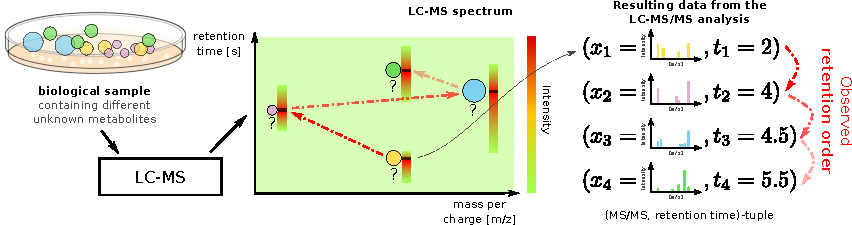
\includegraphics[width=.98\linewidth]{images/lcms_spectrum_complex.pdf}
                    \caption{LC-MS/MS analysis pipeline and resulting data. Observed retention order in \textcolor{red}{red}.}
                    \label{fig:lc_msms_dataset}
\end{figure}    
\end{block}

\begin{block}       {{\normalsize 2. Proposed method: Utilizing observed retention orders}}
\begin{itemize}
                    \setlength\itemsep{0.25em} 
                    \item We propose to use Ranking Support Vector Machine (RankSVM) \citep{Joachims2002} to \textbf{predict the pairwise retention order} of molecular candidate structures.
\begin{itemize}             
                    \vspace{-1.0cm}
                    \item[$\circ$] Retention orders are largely preserved across LC-systems \citep{Stanstrup2015}.
                    \item[$\circ$] RankSVM can be trained on \emph{multiple} retention time datasets arising from \emph{heterogeneous} LC-systems. 
\end{itemize}                    
                    \item We introduce a dynamic programming methodology for \textbf{integrating predicted candidate retention orders and MS/MS based scores} to \emph{jointly} identify a set of metabolites arising, e.g., in a metabolomics experiment (Fig.~\ref{fig:lc_msms_dataset}).
\end{itemize}     
\end{block}

\begin{block}       {{\normalsize 3. Ranking Support Vector Machine (RankSVM)}}
                    
\begin{itemize}
                    \setlength\itemsep{0.25em}
                    \item \textbf{Preference learning} using RankSVM \citep{Joachims2002} for retention order prediction.
                    \item \textbf{Notation}: Molecule $\mol_i$ from molecular space $\molspace$, $t_i\in\rettimespace$ its retention time, $\sys_i$ LC-system it has been measured with. Set of training LC-systems $S$. Set of RTs measured with LC-system $\sys$ is denoted with $\RTimes(s)$.
                    \item Molecule $\mol_i$ is preferred over $\mol_j$ when it elutes before $\mol_j$, i.e. $t_i<t_j$.
                    \item Set of pairwise preferences of LC-system $\sys\in S$ is defined as:                    
\begin{equation}
                    \Pref(s)=\{(i,j)\,|\,s_i = s_j = s,t_i<t_j\} \label{eq:pairwise_preferences_from_system_s}
\end{equation}                    
                    \item Set of pairwise preferences from \emph{multiple} LC-systems:
\begin{equation}
                    \Pref=\bigcup_{\sys \in S}  \Pref(s) \label{eq:pairwise_preferences_from_all_systems}.
\end{equation}                   
                    \item \textbf{Kernel RankSVM}: Molecular structure encoded by kernel function $\kmol:\molspace\times\molspace\rightarrow\mathbb{R}$, with feature-map $\phi:\molspace\rightarrow\Fmol$ and feature space $\Fmol$
                    \item RankSVM preference prediction model: 
\begin{equation}
                    f(\mol_i,\mol_j) = \sgn(\VEC{w}^T(\phi(\mol_j)-\phi(\mol_i)))\in\{-1,1\}
\end{equation}
                    \item Model parameters $\VEC{w}$ are found by solving:
\begin{align}
                    \underset{\VEC{w},\VEC{\xi}}{\min} &\quad \frac{1}{2}\VEC{w}^T\VEC{w} + C\sum_{(i,j)\in  \Pref}\xi_{ij} \\
                    s.t. &\quad\VEC{w}^T(\phi(\mol_j)-\phi(\mol_i))\geq 1-\xi_{ij}, \forall(i,j)\in  \Pref\label{prob:rankSVM-primal}\\
                         &\quad \xi_{ij} \geq 0, \forall(i,j)\in  \Pref,
\end{align}                    
                    with $C>0$ being a regularization parameter. 
                    \item By solving the Problem \eqref{prob:rankSVM-primal}: $\VEC{w}$ is learned such that:
\begin{equation}
                    \VEC{w}^T\phi(\mol_i)<\VEC{w}^T\phi(\mol_j),\,\text{if}\,(i,j)\in  \Pref.\label{eq:prediction_model_RankSVM}
\end{equation}
\end{itemize}
\end{block}

\end{column}
%% <== end of first column

%% Second column ==>
\begin{column}{.52\linewidth}

\begin{block}       {{\normalsize 4. Integration of MS/MS scores \& retention orders}}
\begin{itemize}
                    \setlength\itemsep{0.25em}
                    \item \textbf{Notation}: $n_{i,j}$ denotes molecular candidate $j$ for spectrum $i$ and $y_{i,j}$ its MS/MS based score.
                    \item MS/MS scores predicted using Input Output Kernel Regression (IOKR) \citep{Brouard2016}
                    \item Directed graph $G$ with nodes representing the molecular candidates (Fig.~\ref{fig:dynamic_programming})
                    \item Edges connect the candidates $n_{i,j}$ and $n_{i+1,s}$ with weight:
\begin{equation}
                    \delta_{(i,j),(i+1,s)}=-y_{i+1,s}+D\cdot\max(0,\mathbf{w}^T(\phi(m_{i,j})-\phi(m_{i+1,s})),
\end{equation}                     
                    $D\geq 0$ weight on order penalty: $\max(\ldots)>0$ if observed $\neq$ predicted order.
                    \item Molecular candidates along the \textbf{shortest path} connecting the first and the last layer are the \textbf{most consistent identifications}.
\end{itemize}
\begin{figure}
                    \centering
                    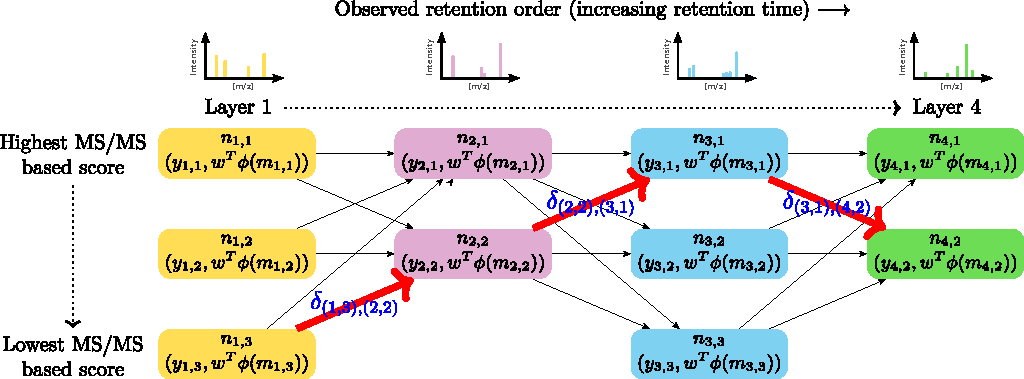
\includegraphics[width=.98\textwidth]{images/dynamic_programming_simple_2.pdf}
                    \caption{$G$ with layers corresponding to the molecular candidates per MS/MS. Shortest path in \textcolor{red}{red}.}
                    \label{fig:dynamic_programming}
\end{figure}
\end{block}

\begin{block}       {{\normalsize 5. Experiments}}
                    \textbf{Retention order prediction:}
\begin{itemize}
                    \setlength\itemsep{0.25em}
                    \item 1098 retention times from 5 different reversed phase LC-systems \citep{Stanstrup2015} ($\hat{S}$)
                    \item Molecular representation: Counting fingerprints based on the MACCS dictionary \citep{Durant2002} combined with MinMax-Kernel \citep{Ralaivola2005} $\kmol$
                    \item Competing method: Retention time predicting using Support Vector Regression (SVR) \citep{Aicheler2015}.
                    \item Access prediction accuracy in target system $\sys\in\hat{S}$ by cross-validation (Fig.~\ref{fig:all_on_one_vs_baseline})
                    \item Training sets for RankSVM and SVR for target LC-system $\sys\in \hat{S}$: 
\begin{table}
                    \centering
\begin{small}
\begin{tabular}{l|c|c}
                    \toprule
                    Single (only target) system & $\Pref(\sys)$ \hfill (RankSVM) & $\RTimes(\sys)$ \hfill (SVR) \\
                    Multiple (all available) systems & $\bigcup_{\sys \in \hat{S}} \Pref(s)$ \hfill (RankSVM) & $\bigcup_{\sys \in \hat{S}} \RTimes(\sys)$ \hfill (SVR)\\
                    \bottomrule
\end{tabular}
\end{small}                    
\end{table}   
\end{itemize}
                    \textbf{Metabolite identification:}
\begin{itemize}
                    \setlength\itemsep{0.25em}
                    \item 342 reversed phase LC RTs: for 120 MS/MS spectra available $\rightarrow$ (MS/MS, RT)-tuple, remaining 222 used for RankSVM training ($\sys_{Impact}$)
                    \item Identification performance for different $D$ values accessed using repeated bootstrapping of 80 tuples (Fig.~\ref{fig:top1_acc_for_different_D}, black line: baseline with $D=0$)
                    \item Different RankSVM training sets:
\begin{small}
\begin{tabular}{l|c|c}
                    \toprule
                    (only) Target & $\Pref(\sys_{Impact})$ & 222 Mol.\\
                    (only) Others & $\bigcup_{\sys \in \hat{S}} \Pref(s)$ & 1098 Mol.\\
                    Others \& target & $\bigcup_{\sys \in \hat{S}} \Pref(s) \cup \Pref(\sys_{Impact})$ & 1320 Mol.\\
                    \bottomrule
\end{tabular}
\end{small}                      
%\begin{table}
%                    \centering
%                  
%\end{table}                     
\end{itemize}                    
\begin{columns}
\begin{column}{.01\linewidth}
\end{column}
\begin{column}{.49\linewidth}
\begin{figure}
                    \centering
                    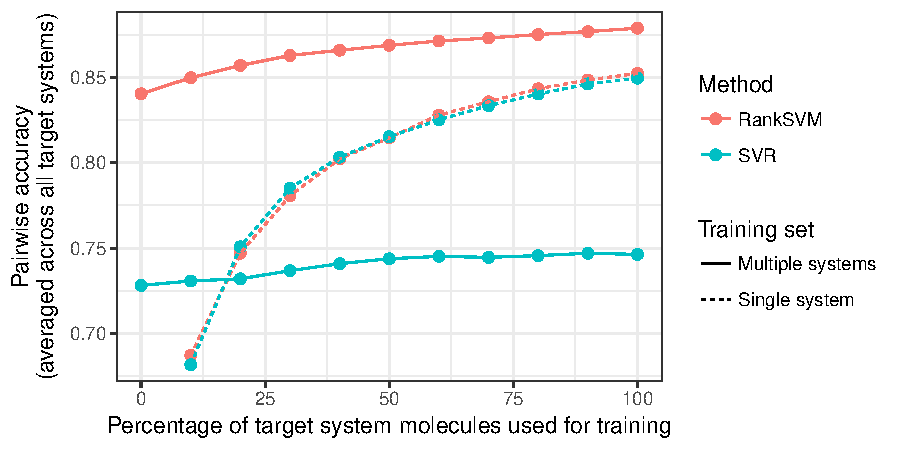
\includegraphics[width=\textwidth]{images/pwacc_avg_across_systems_all_on_one_perc_2.pdf}
                    \caption{Accuracy averaged over the 5 systems.}
                    \label{fig:all_on_one_vs_baseline}
\end{figure}
\end{column}
\begin{column}{.49\linewidth}
\begin{figure}
                    \centering
                    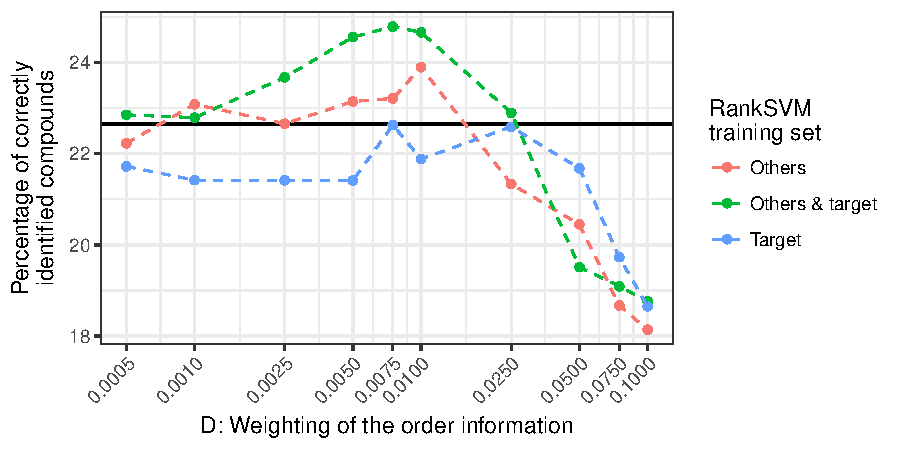
\includegraphics[width=\textwidth]{images/top1_accuracy_reranking_GS_BS_n_rep=1000_no_facet.pdf}
                    \caption{Accuracy averaged over 1000 samples.}
                    \label{fig:top1_acc_for_different_D}
\end{figure}
\end{column}
\begin{column}{.01\linewidth}
\end{column}
\end{columns}                    
\end{block}

\vfill

\begin{block}       {\small References}
\bibliographystyle  {abbrv}
\vspace{-1.5cm}
\begin{multicols}{2}
\begin{footnotesize}
\bibliography       {biblib.bib}
\end{footnotesize}
\end{multicols}
\end{block}

\end{column}
%% <== end of second column

\end{columns}

\vfill

\end{frame}
\end{document}
